\subsection{Justification Analysis}

One challenge that we had through the project were to implement a low-pass filter to get smooth moving bars. During the design part we spent a lot of time thinking of how to do this and calculating math.

The incoming signals are low-pass filtered with a saturation time of approximately 100 ms (4096 sample cycles) as seen in figure \ref{fig:lowpass}, resulting in a measurement of the signal's power. 

\begin{figure}[h]
\centering
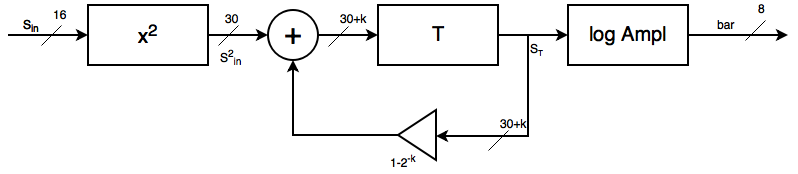
\includegraphics[width=16cm]{lowpass}
\caption{The low-pass filter. $k$ is chosen by the approximation $\frac{1}{10}\mathrm{\ s} = 2^k\cdot\frac{1}{48800}\Rightarrow 2^k=4880\approx 2^{12}\Rightarrow k = 12 $}
\label{fig:lowpass}
\end{figure}


\verb=log_Pow= takes the logarithm of the low-pass filtered signal. It provides module outputs proportional to the result, updating only in sync with \verb+vsync+. The \verb+bar+ signals are lined to \verb+VGA_Driver+ as definitive information about how the power bars should render on screen.

